\documentclass{article}
\usepackage[utf8]{inputenc}
\usepackage{pdfpages}

\author{Accordi Gianmarco}
\title{Reverse Engineering}

\usepackage{natbib}
\usepackage{graphicx}
\usepackage{minted}
\usepackage{tabularx}
\usepackage{tikz}
\usepackage{pgfplots}
\usepackage{hyperref}

\usemintedstyle{fruity}
\date{}

\begin{document}

\maketitle

\section{Introduction}

\textbf{Reverse Engineering} is the process of understanding how system made by man is working, by looking at it an trying to reverse the operations it does in order to understand its behavior.
Its like a scientific research but in this case we are not interested in natural phenomenon.
This kind of process has been applied to a lot of different fields, from mechanical engineering to chemical engineering, so as the name suggested it is applied to all field of engineering: these are the fields in which we can take apart the work done by other human being and trying to understand how they have build such a system.
The necessity of this such an analysis of a system is usually required because creator of a system tends to disclose how they've built it, this mean that they obscure their work in order to protect their creators rights.
The purpose of this document is to give an introduction on \textbf{Reverse Engineering} specifically in the field of Software Engineering.
The process of Reverse Engineering applied to Software products can be done at any level of the production, but it usually involves two stages \footnote{\url{https://en.wikipedia.org/wiki/Reverse_engineering}}:
\begin{itemize}
    \item \textbf{Redocumentation}: since usually the given software product that we want to analyze is already compiled we want to be able to reach an higher level of abstraction to better understand the code;
    \item \textbf{Design Understanding}: once that we have been able to get an higher abstraction of our code we can use our capacity and knowledge in order to understand what the program does and how it does it, so we want to follow the development process of the creators of such code.
\end{itemize}
Disclose the design features can be understand with two approaches:
\begin{itemize} 
    \item \textbf{Dynamic Analysis}: this is an on the field approach, in which you launch the program and you register what the program is doing, and by analyzing the impact it has on the environment(print,systemcalls,...) you try to figure out what it does;
    \item \textbf{Static Analysis}: analyze the code without launch it, you analyze only the output you've obtained from the \underline{Redocumentation} part.
\end{itemize} 
In next sections we will analyze this approaches along with the stage involved in doing them.
Then we proceed in order to define which is the best strategy based on what we have seen. Finally an example is provided taken from a CTF. 

\subparagraph{Reverse Engineering in Software Engineering}
As previously stated this document focus its attention on Reverse Engineering applied to software. When a new software is released it is usually provided already compiled to the specific architecture, so you get the binary of this code.
The binary, as the name suggests, contains binary instructions that are targeted to be understood by a specific machine with a specific architecture, this means that it cannot be understand easily from a human being.
For the developers this is usually a wanted feature, since this make the reverse engineering process more difficult for other companies that wants to disclose their design features.
To be even more secure companies also rely on the usage of some \underline{Obfuscation Technique} that makes the reverse engineering process even harder. This leads to the development of new research fields focused on trying to remove obfuscation, also in an automate way \citep{1566145}.
Some techniques used for obfuscate binaries are Packing( in which the source code pack and unpack the .text section as long as it execute)\citep{SlidePackers}, Dynamic Code Mutation( in which the code mutate during execution), Code Generation( the program generates code during program execution) or by Binary Instumentation \cite{paperInstrumentation}.
So in the end software is usually not fully disclose for two main reasons: protection of intellectual property and malware. In next sections we will see different techniques that can be used in order to defeat make the process of reverse engineering more easy.

\clearpage

\section{Stages} 
The process of \textbf{Reverse Engineering} pass through 2 main stages, the \underline{Redocumentation} part analysis statically the executable starting from a decompilation process.
while the second part called \underline{Design Understanding} involves the outcome of the previous stage combined with dynamic analysis, based on the strategy we choose to adopt. 

\subsection{Redocumentation}
\label{section:redocumentation}
The program we get is usually a binary file so the first steps in order to get an higher level representation of it is to disassemble it.
\begin{figure}[htp]
    \centering
    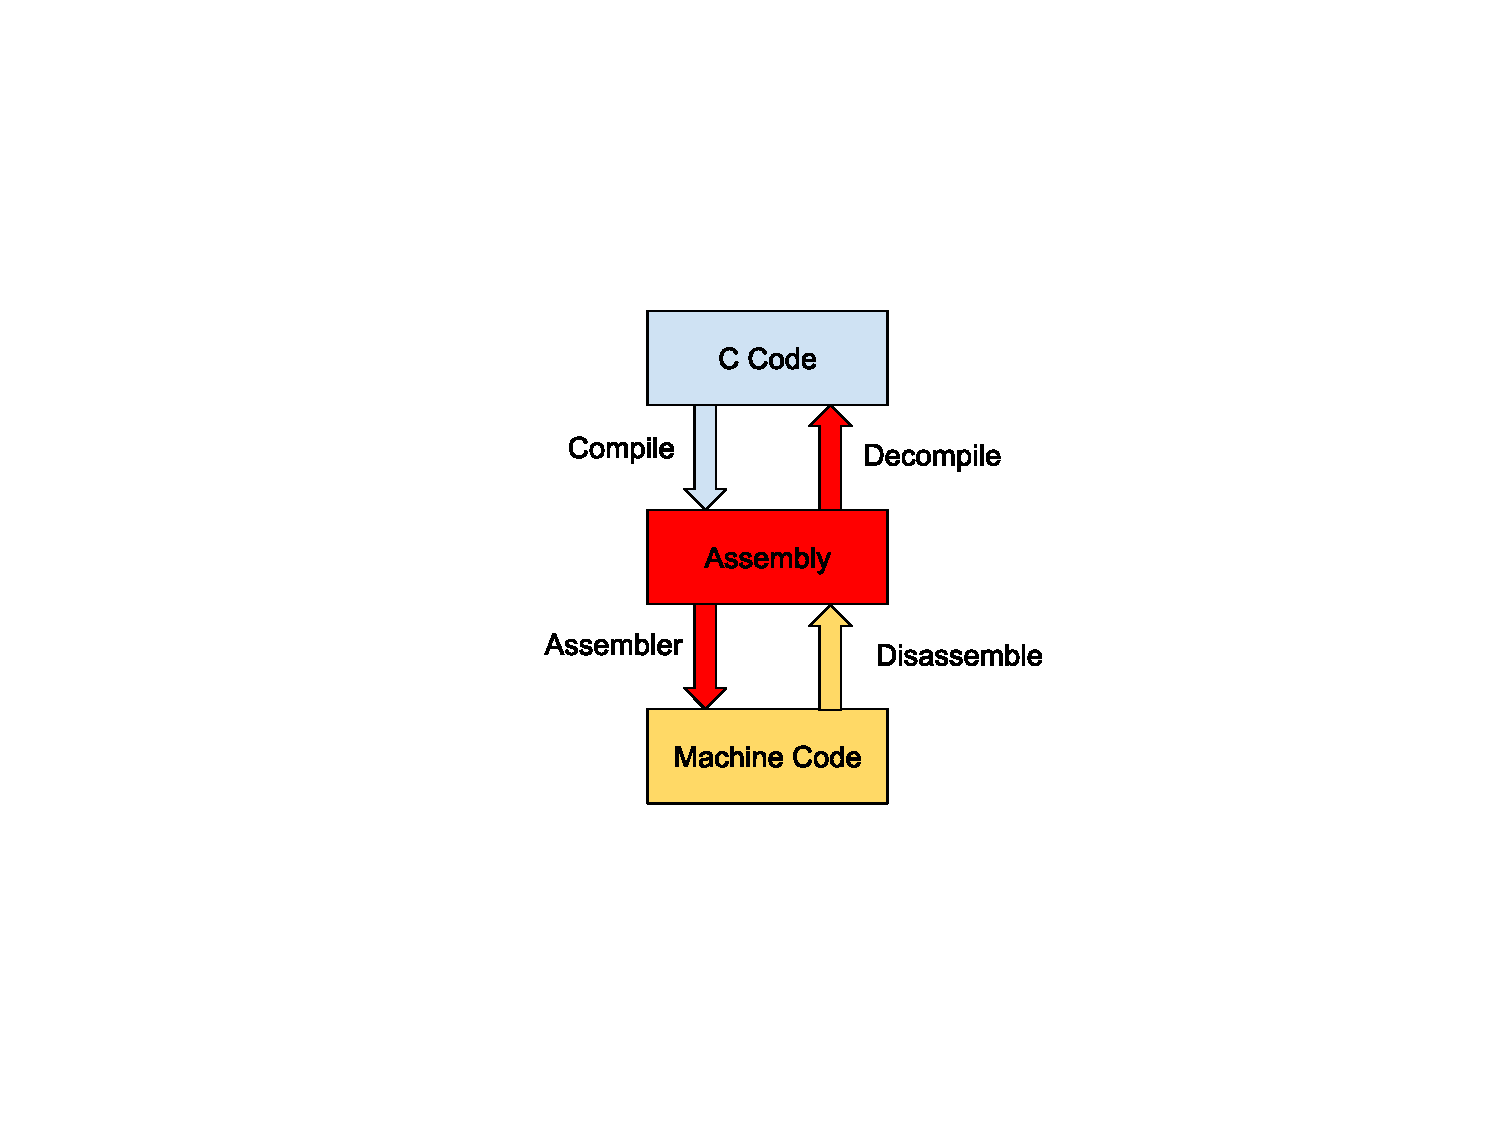
\includegraphics[width=1\textwidth]{images/redocumentation.pdf}
    \caption{Compilation and Decompilation steps \citep{SlideReverse}}
    \label{fig:redocumentation}
\end{figure}
Figure \ref{fig:redocumentation} refers to the case of compiled languages( and we will refers to the them from now on), as we can see when someone wants to make its code executable has to go throw a set of steps usually:
\begin{itemize}
    \item \textbf{Compilation}: from the high level code( say for example C code) you use the compiler \footnote{\url{https://en.wikipedia.org/wiki/Compiler}} to generate a low level language that usually is Assembly code;
    \item \textbf{Assembler}: in this stage you pass from Assembly code, that has an high correspondence with the machine code instructions so it is targeted to a specific architecture \footnote{\url{https://en.wikipedia.org/wiki/Assembly_language}}, into machine code that can be executed.
\end{itemize}
In fact what we usually have is the machine code, the executable file. From it we have to extract useful information to understand what it does, this again requires to revert the previous operations, as shown in \ref{fig:redocumentation}( going down to up):
\begin{itemize}
    \item \textbf{Disassemble}: from the machine code of a specific architecture(that can be x86-64 or arm) we get the correspondent Assembly code;
    \item \textbf{Decompile}: from the assembly code we have obtain our aim is to get the high level source code that has generate it as similar as possible to the original one.
\end{itemize}
The process of generating an executable is not an invertible function \footnote{\url{https://en.wikipedia.org/wiki/Decompiler}} This means that by doing so we lost some information, that makes the inverse process quite harder.
In fact the output of the decompilation stage can vary based on the compiler used to perform compilation and the presence of metadata present inside of the executable, if for example has been included debug information or if instead it has been stripped of all the metadata. The outcome of the compilation change also based on the optimization enabled at compile time.
As previously state some code can also be harder to be decompiled since it has been obfuscated with different techniques, another example is the insertion of instructions that doesn't change the flow of executed instructions but it insertion broke the alignment and so the decompiler is not able to recognize instructions in the correct way.
The \underline{output of the Disassemble stage} can be analyzed as shown in figure \ref{fig:decompilationoutput}. We can organize block of assembly instructions inside block that are executed sequentially, until some instruction that controls the execution flow are encountered, like jump instruction.
In such cases the flow is divided into different block of other assembly instructions.
\begin{figure}[htp]
    \centering
    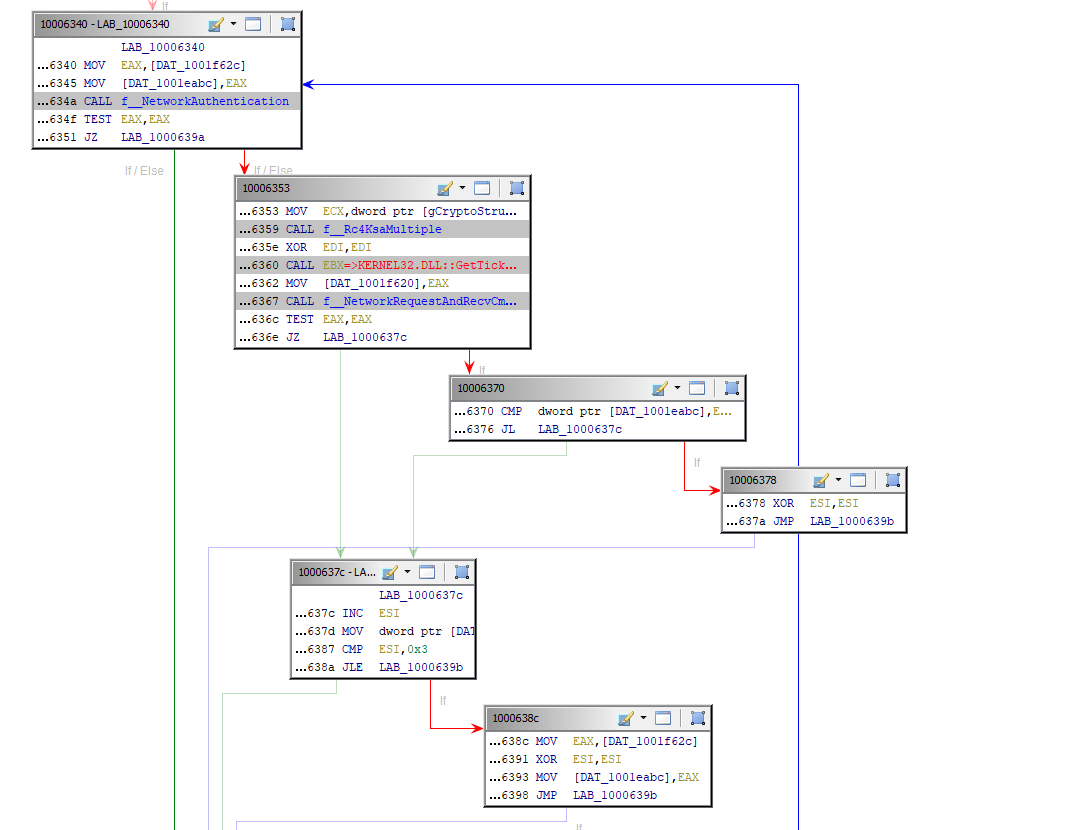
\includegraphics[width=1\textwidth]{images/graphview.png}
    \caption{Analysis of the Decompilation's output stage.}
    \label{fig:decompilationoutput}
\end{figure}
The output of the Decompilation part can be read mode easily since it will be something similar to the original source code that has produced the executable file. 
\begin{figure}[htp]
    \centering
    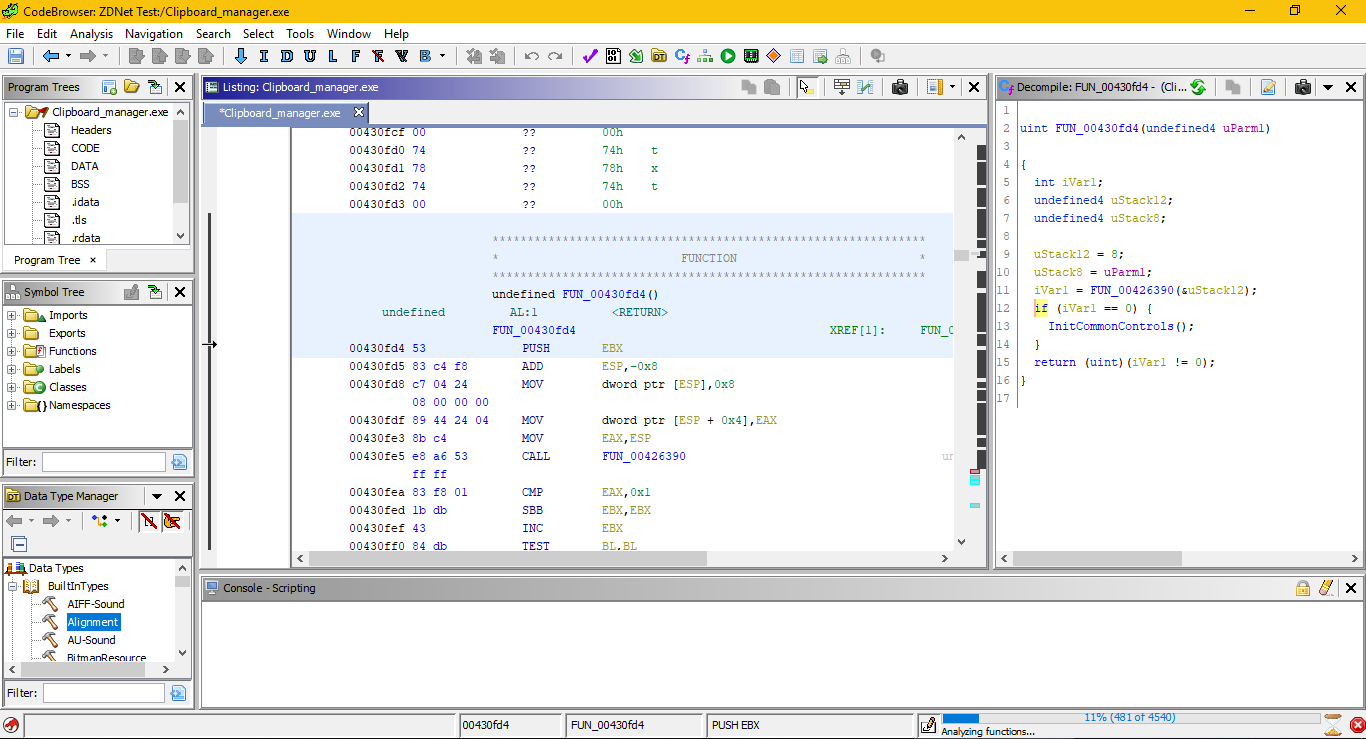
\includegraphics[width=1\textwidth]{images/ghidra.png}
    \caption{Ghidra GUI after analyzing an executable file.}
    \label{fig:ghidraoutput}
\end{figure}
The readability of the output depends on the quality of the tool used to decompile and on the present metadata, but it is more than recommended a user inspection of code, for example to better understand the type of the variable.
\begin{figure}[htp]
    \centering
    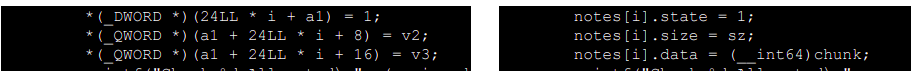
\includegraphics[width=1\textwidth]{images/coderead.png}
    \caption{Code readability after inspection of the struct.}
    \label{fig:coderead}
\end{figure}
As you can see in image \ref{fig:coderead} the code on the right is more readable after inspection if the code, and the definition of a strut hat better fits the memory structure that is used by the executable.
Up to know we have assumed to have under analysis an executable from a \textit{Compiled Language}, but the same things can be applied to \textit{Interpreted Language} \footnote{\url{https://en.wikipedia.org/wiki/Compiled_language}} like for example Java, in which some tool exists in order to analysis the bytecode produced by java \footnote{\url{http://java-decompiler.github.io/}}.
The work done during this stage is important in the first strategy that we will purse in order to discover design features of the programs under analysis: \underline{Static Analysis}.

\clearpage

\subsection{Design Understanding}
The objective of the Reverse Engineering task is to understand the \textit{Design Features} of the program under analysis. So in order to reach this results one can use different techniques, that can be generalized into two main categories: \textbf{Static Analysis} and \textbf{Dynamic Analysis}.

\paragraph{Static Analysis}
What we have seen during the \textit{Redocumentation} stage \ref{section:redocumentation} is what we can think as Static analysis, in fact it is the process of code analysis without regard of its execution or input \citep{LessonReverse}.
From this analysis we can take a look at the:
\begin{itemize}
    \item \textbf{Control flow}: the code is broke down into block, that merged together instructions that will be executed sequentially, this separation in block can be done by looking at how the control instructions are placed, like if or while loop \ref{fig:decompilationoutput}, in this way we can try to understand which is the path block executed by the program sequentially, so we can follow the execution flow;
    \item \textbf{Data Flow}: helps in understanding how the data flows inside the program, from the input we can give to the program to the final outcome of its execution.
\end{itemize}
//TODO

\paragraph{Dynamic Analysis}
Opposed to Static the Dynamic Analysis instead rely on the execution of the program regarding on the input provided to it. In this case we try to launch the executable with different inputs and look at the different outcome we got.
\begin{figure}[htp]
    \centering
    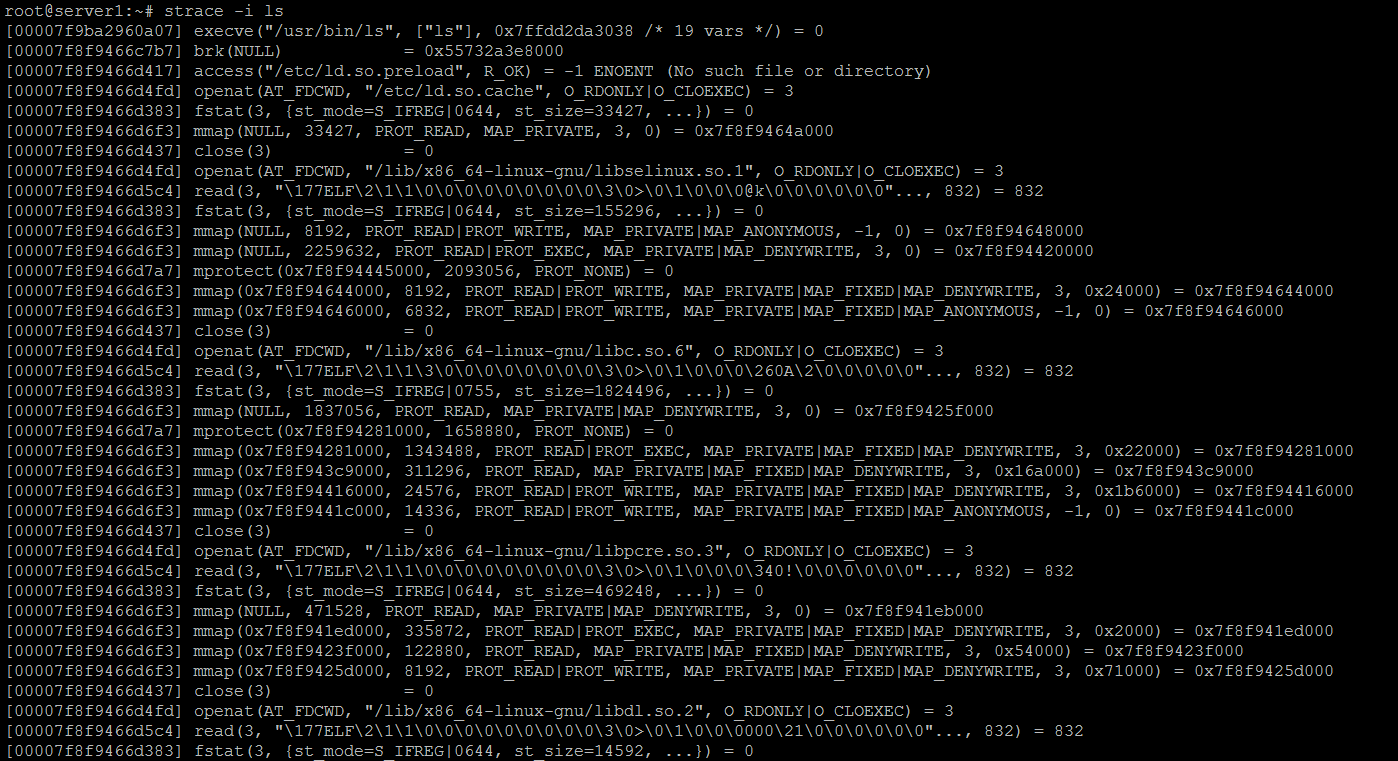
\includegraphics[width=1\textwidth]{images/strace.png}
    \caption{The possible output of strace after an executable execution.}
    \label{fig:strace}
\end{figure}
And by looking at the output returned by the executable we try to guess what the program does. We can also use some other tools to understand what the executable does by looking at the system calls invocation done by it, in this case we can user \textit{strace}\footnote{\url{https://en.wikipedia.org/wiki/Strace}}. As we can see in figure \ref{fig:strace} the output will make a summary of the various system calls done by a certain program.
\textit{Strace} allows to analysis how the executable access to the privileged kernel mode, how the program switch its execution from user mode to kernel mode. Other tools that can be used are \textit{ltrace} and \textit{ptrace}.

//TODO introduce debugger

//TODO make another section with an image with the relation between static and dynamic analysis, and how to use them togheter

\subsection{Example of code}
Here you can fine an example of how to add some code. It is using the package minted with basic option enabled.
You can write code in place:
\begin{minted}[linenos, bgcolor=black, escapeinside=!!]{python}
import numpy as np
    
def incmatrix(genl1,genl2):
    m = len(genl1)
    n = len(genl2) !\label{myline}!
    M = None #to become the incidence matrix
    VT = np.zeros((n*m,1), int)  #dummy variable
    
    #compute the bitwise xor matrix
    M1 = bitxormatrix(genl1)
    M2 = np.triu(bitxormatrix(genl2),1) 
...
\end{minted}
You can reference to a line
The important line is line \ref{myline}.

You can use an external file and ave the code as listing.
\begin{listing}[ht]
\inputminted[linenos, bgcolor=black, escapeinside=!!]{python}{x.py}
\caption{Example from external file}
\label{listing:3}
\end{listing}
 
The important line is line \ref{anotherline} of Listing~\ref{listing:3}.

\section{Conclusion}


\bibliographystyle{plain}
\bibliography{references}
\end{document}
